% This is based on the LLNCS.DEM the demonstration file of
% the LaTeX macro package from Springer-Verlag
% for Lecture Notes in Computer Science,
% version 2.4 for LaTeX2e as of 16. April 2010
%
% See http://www.springer.com/computer/lncs/lncs+authors?SGWID=0-40209-0-0-0
% for the full guidelines.
%

\documentclass{llncs}

\usepackage[utf8]{inputenc}
\usepackage[T1]{fontenc}
\usepackage[polish]{babel}
\usepackage[colorinlistoftodos]{todonotes}
\usepackage{hyperref}
\usepackage{subfig}
\usepackage{listings}
\usepackage{float}

\usepackage{color}
\usepackage{courier}
 
\definecolor{codegreen}{rgb}{0,0.6,0}
\definecolor{codegray}{rgb}{0.5,0.5,0.5}
\definecolor{codepurple}{rgb}{0.58,0,0.82}
\definecolor{backcolour}{rgb}{0.95,0.95,0.92}
 
\lstdefinestyle{mystyle}{
    backgroundcolor=\color{backcolour},   
    commentstyle=\color{codegreen},
    numberstyle=\tiny\color{codepurple},
    stringstyle=\color{codepurple},
    basicstyle=\footnotesize\ttfamily,
    breakatwhitespace=false,         
    breaklines=true,                 
    captionpos=b,                    
    keepspaces=true,                 
    numbers=left,                    
    numbersep=5pt,                  
    showspaces=false,                
    showstringspaces=false,
    showtabs=false,                  
    tabsize=2
}
 
\lstset{style=mystyle}

\begin{document}

\title{Konwolucyjna sieć neuronowa grająca w Connect4}
%
\titlerunning{ConvConnect4}  % abbreviated title (for running head)
%                                     also used for the TOC unless
%                                     \toctitle is used
%
\author{Tomasz Janiszewski\inst{1} \and Jakub Dutkowski\inst{2}}
%
\authorrunning{Tomasz Janiszewski, Jakub Dutkowski} % abbreviated author list (for running head)
%
%%%% list of authors for the TOC (use if author list has to be modified)
\tocauthor{Tomasz Janiszewski and Jakub Dutkowski}

\institute{Politechnika Warszawska\\
Wydział Matematyki i Nauk Informacyjnych
\email{janiszewskit@student.mini.pw.edu.pl}~~
\email{dutkowskij@student.mini.pw.edu.pl}}

\maketitle              % typeset the title of the contribution

\keywords{Connect4, Convolutional Neural Network, Deep learning, cognitive approach,
intuitive playing, human-like problem solving, example-based learning, Connect Four.}
%
\section{Wstęp}
Celem projektu było stworzenie rozwiązania znajdującego optymalny ruch (bądź jego przybliżenie) w grze Connect Four (\emph{pol. Czwórki}) \cite{connect4:wiki} na podstawie obrazu planszy, bez przeszukiwania drzewa gry. 
W trakcie trawania projektu przetestowano dwa różne modele
\begin{enumerate}
	\item konwolucyjną sieć neuronową złożona z wielu perceptronów
	\item sieć Kohonena uczoną z nadzorem
\end{enumerate}

\section{Model perceptronowy}

\subsection{Reprezentacja planszy}
\label{sec:reprezentacja}
Aby wykorzystać lokalność kontekstu gry, plansza do gry podzielona będzie na nachodzące na siebie sektory - kwadraty $4 \times 4$ (jak na \autoref{fig:C4Podzial}). 
Każdy z kwadratów reprezentowany będzie jako wektor szesnastu liczb $\{-1, 0, 1\}$, gdzie:
\begin{description}
	\item[1] oznacza krążęk gracza aktywnego
	\item[-1] oznacza krążek gracza nieaktywnego
	\item[0] oznacza puste pole
\end{description} 

Wartości odpowiadające polom w sektorze ustawione będą kolejno jak na \autoref{fig:C4Kolejnosc}. Kolejne sektory będą numerowane kolumnami, od góry do dołu, od lewej do prawej.

\begin{figure}[H]
	\centering	
	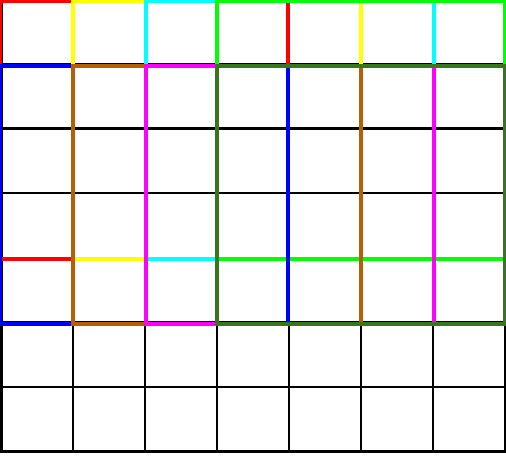
\includegraphics[width=0.5\textwidth]{img/ConnectFour4x4.pdf}
	\caption{Podział planszy na kwadraty 4x4. Dla czytelności, przedstawiono tylko pierwsze dwa wiersze.}
	\label{fig:C4Podzial}
\end{figure}

\begin{figure}[H]
	\centering	
	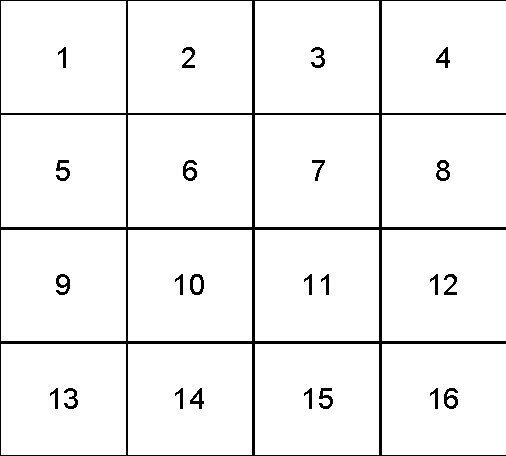
\includegraphics[width=0.5\textwidth]{img/ConnectFourOrder.pdf}	\caption{Kolejność pól w wektorze kodującym sektor planszy.}
	\label{fig:C4Kolejnosc}
\end{figure}

\subsection{Opis sieci}
Wejście sieci składało się z $16 \times 16$ neuronów - po jednym neuronie na każde z $16$ pól w każdym z $16$ sektorów. Części odpowiadające kolejnym sektorom miały związane odpowiednie wagi (np. waga odpowiadająca polu nr 1 w sektorze I związana z wagą pola nr 1 w sektorze nr III). Kolejna warstwa składała się z $4 \times 16$ neuronów - po jednym na każdą kolumnę każdego z sektorów.
Wyjście tej warstwy złożnoe z $4 \times 4$ neuronów, odpowiadającym kolumną planszy w każdej \emph{kolumnie sektorów}. Podobnie jak w przypadku 
poprzedniej warstwy, poszczególne elementy odpowiadające kolumną sektorów miały związane wagi.
Wyjście sieci składało się będzie z siedmiu neuronów odpowiadających kolumnom na planszy. Największa wartość oznacza numer kolumny w następnym ruchu.
Wszystkie połączenia pomiędzy warstwami jak na \autoref{fig:Siec}

\begin{figure}[H]
	\centering	
	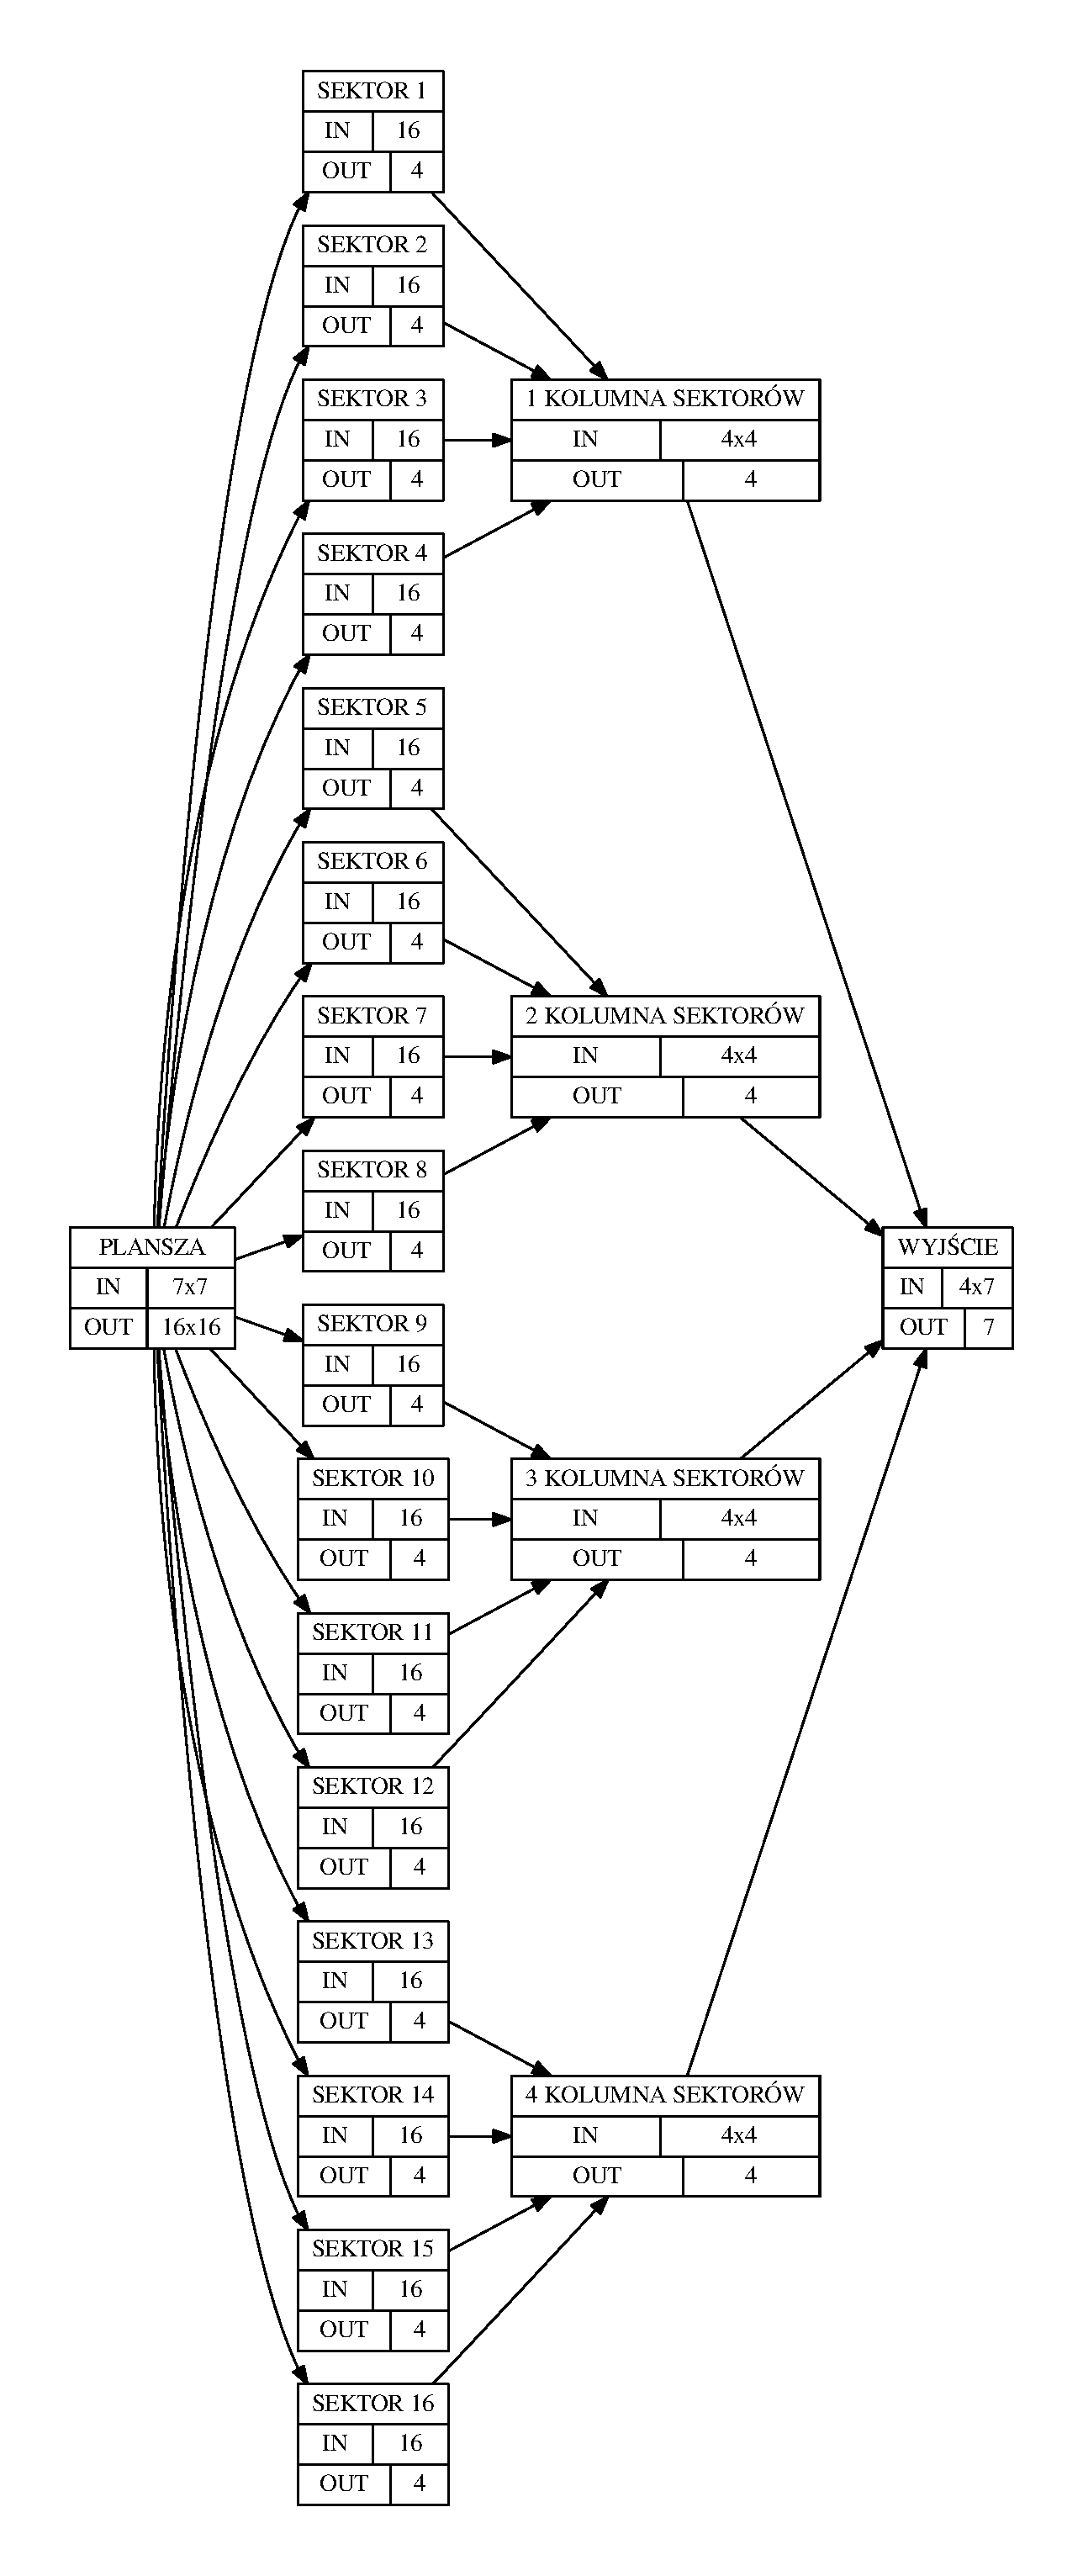
\includegraphics[width=0.5\textwidth]{img/opis_sieci.pdf}	\caption{Budowa sieci.}
	\label{fig:Siec}
\end{figure}

\subsection{Algorytm uczenia i grania}
Sieć będzie uczona za pomocą algorytmu propagacji wstecznej. Dane treningowe wygenerowane zostaną za pomocą programu Velena\cite{velena} wykonującego perfekcycjne ruchy.

\subsection{Wyniki}
Otrzymane rezultaty nie były zadowalające. Skuteczność przewidywania liczona jako procent ruchów równych tym przewidzianym przez Velenę wynosiła około $20\%$ (zupełnie losowe ruchy dają skuteczność na poziomie $18\%$).

\section{Model Kohonena}

\subsection{Opis modelu}
W drugim podejściu postaniowiono użyć zmodyfikowanej sieci Kohonena. Sieć Kohonena pozwala na zdyskretyzowanie przestrzeni wejściowej i jest uczona bez nadzoru.
W niniejszej pracy rozszerzono model o uczenie nadzorowane tak aby sieć zamieniała konkretny obraz planszy na jeden z możliwych ruchów.

\subsection{Opis wejścia}
Na wejściu znajduje sie wektor o rozmiarze $6\times 7$ elementów reprezentujący stan planszy. Kodowanie jest identyczne jak w poprzednim modelu (\autoref{sec:reprezentacja}).

\subsection{Opis sieci}
Sieć jest zbudowana z $6$ neuronów, z których każdy jest połączony wagami z każdym elementem wektora wejściowego. 
Każdy neuron ustala swoje wagi. Wyjściem sieci jest indeks neuronu który zwrócił najwyższy wynik.

\subsection{Algorytm uczenia}
Skorzystano z algorytmu uczenia z nadzorem. Wagi każdego z neuronów są zawsze znormalizowane podobnie jak wektor wejściowy.
Uczenie polega na zmianie wag neuronu, którego indeks jest porządanym ruchem tak, aby jego wynik był największy, w myśl zasady
zwycięzca bierze wszystko.


\begin{lstlisting}[language=Octave,frame=single,caption=Implementacja algorytmu w języku Octave]
global WIDTH = 7;
global HEIGHT = 6;
global INPUTS = WIDTH*HEIGHT;

for iteration = 1:ITERATIONS
  RATE = 1 / (1+iteration);
  for example_index = 1:size(examples)
    example = examples(example_index, :);
    from = 1+(answers(example_index))*INPUTS;
    to = (answers(example_index)+1)*INPUTS;
    weights(from:to) = normalize(weights(from:to) + RATE*(example-weights(from:to)));
  endfor
endfor
\end{lstlisting}
\begin{lstlisting}[language=Octave,frame=single,caption=Implementacja normalizacji w języku Octave]
function normalized = normalize(x)
  if ~isvector(x)
      error('Input must be a vector')
  end
  normalized = x./sqrt(sum(x.^2));
  normalized(!isfinite(normalized))=0;
end
\end{lstlisting}
W powyższym algorytmie na wynik uczenia wpływ ma zmienna \texttt{RATE}, która określa jak duże zmiany są nakładane na wagi.

\subsection{Wyniki}
Dziłanie algorytmu zostało przetestowane dla różnych wartości parametru \texttt{RATE}. Próbę przeprowadzono na 
losowo wybranych planszach. Zbiory treningowy i testowy miały rozmiar $150~tys$ elementów.

\begin{figure}[H]
	\centering	
	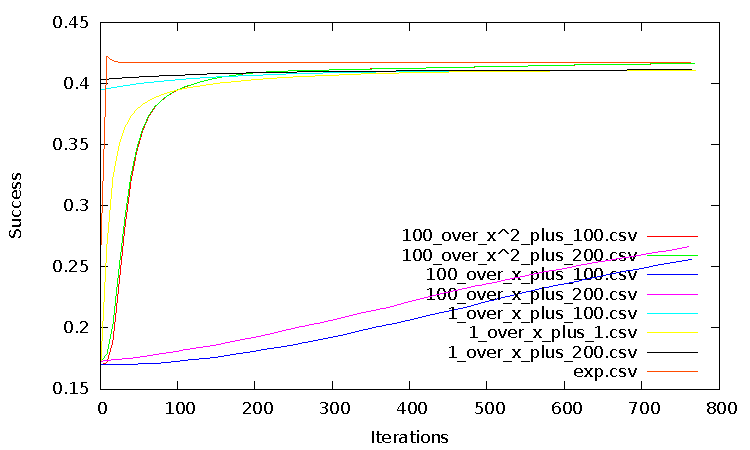
\includegraphics[width=\textwidth]{img/test}	\caption{Skuteczność na zbiorze testowym.}
	\label{fig:Siec}
\end{figure}

Ciekawym zjawiskiem jest pojawienie artefaktu, w okolicach którego skuteczność bardzo gwałtownie się zmienia.
Występuje on zarówno dla danych testowych jaki i treningowych.
Otrzymywana skuteczność to około $40\%$.



%
% ---- Bibliography ----
%
\begin{thebibliography}{4}
%
\bibitem {mandziuk2011}
Mandziuk, J.:
\textsl{Towards Cognitively Plausible Game Playing Systems}
IEEE COMPUTATIONAL INTELLIGENCE MAGAZINE, Maj, 2011
\bibitem {Ah-Hwee}
Ah-Hwee Tan
\textsl{FALCON: A Fusion Architecture for Learning, COgnition, and Navigation}
\bibitem {webinar}
Yann LeCun
\textsl{Gtc Express Convolutional Networks Webinar}
\url{http://on-demand.gputechconf.com/gtc/2014/webinar/gtc-express-convolutional-networks-webinar.mp4}
\bibitem {connect4:wiki}
\textsl{Connect Four --- {W}ikipedia{,} The Free Encyclopedia}
\url{http://en.wikipedia.org/wiki/Connect_Four}
\bibitem {velena}
\textsl{A Shannon C-type program which plays connect four perfectly}
\url{http://www.ce.unipr.it/~gbe/velena.html}
\end{thebibliography}

\end{document}
